\chapter{Tätigkeitsbereiche und Aufgaben}
\label{sec:main}
\section{Überblick}
\label{sec:main:overview}
Ich habe im Rahmen meines Praktikums am Projekt \textit{SD4M - Smart Data for Mobility} mitgearbeitet.
Meine konkrete Aufgabe war die Aufbereitung und Integration verschiedener Daten und Datenbanken, damit diese im Projekt Verwendung finden können. Meine Hauptdatenquelle waren die Geodaten des OpenStreetMap\footnote{http://www.openstreetmap.org/} Projekts.
\subsection{Das Projekt SD4M}
\label{sec:main:overview:sd4m}
Das Projekt \textit{Smart Data for Mobilty}\footnote{http://sd4m.net/}, im folgenden \textit{SD4M} genannt, ist ein Verbundprojekt eines Konsortiums aus 5 Partnern und wird vom Bundesministerium für Wirtschaft und Energie gefördert.
Das Konsortium besteht aus 4 Wirtschaftsunternehmen und dem DFKI als Forschungseinrichtung.
\begin{compactitem}
  \item DB Systel GmbH (Konsortialführung)
  \item Deutsches Forschungszentrum für Künstliche Intelligenz GmbH
  \item idalab GmbH
  \item ]init[ AG für digitale Kommunikation
  \item PS-Team Deutschland GmbH & Co. KG
\end{compactitem}
Ziel des SD4M Projekts ist eine branchenübergreifende Serviceplattform, welche Daten der unterschiedlichen Mobilitätsanbieter (z.B. der Fahrplan der Deutschen Bahn) sowie öffentliche verfügbare strukturierte und unstrukturierte Daten (z.B. Twitter oder Facebook) miteinander verknüpft.
Diese verknüpften Daten sind für Endnutzer, aber auch für Unternehmen oder die öffentliche Verwaltung von Interesse.
In Abbildung \ref{fig:tweetXfahrplan} wird verdeutlicht, wie sich aus unstrukturierten Twitter-Daten Verspätungsinformationen für konkrete Verkehrsmittel extrahieren lassen.
Diese können dann Endnutzern oder den Mobilitätsanbietern zur Verfügung gestellt werden.
\begin{figure}
   \centering
   \fbox{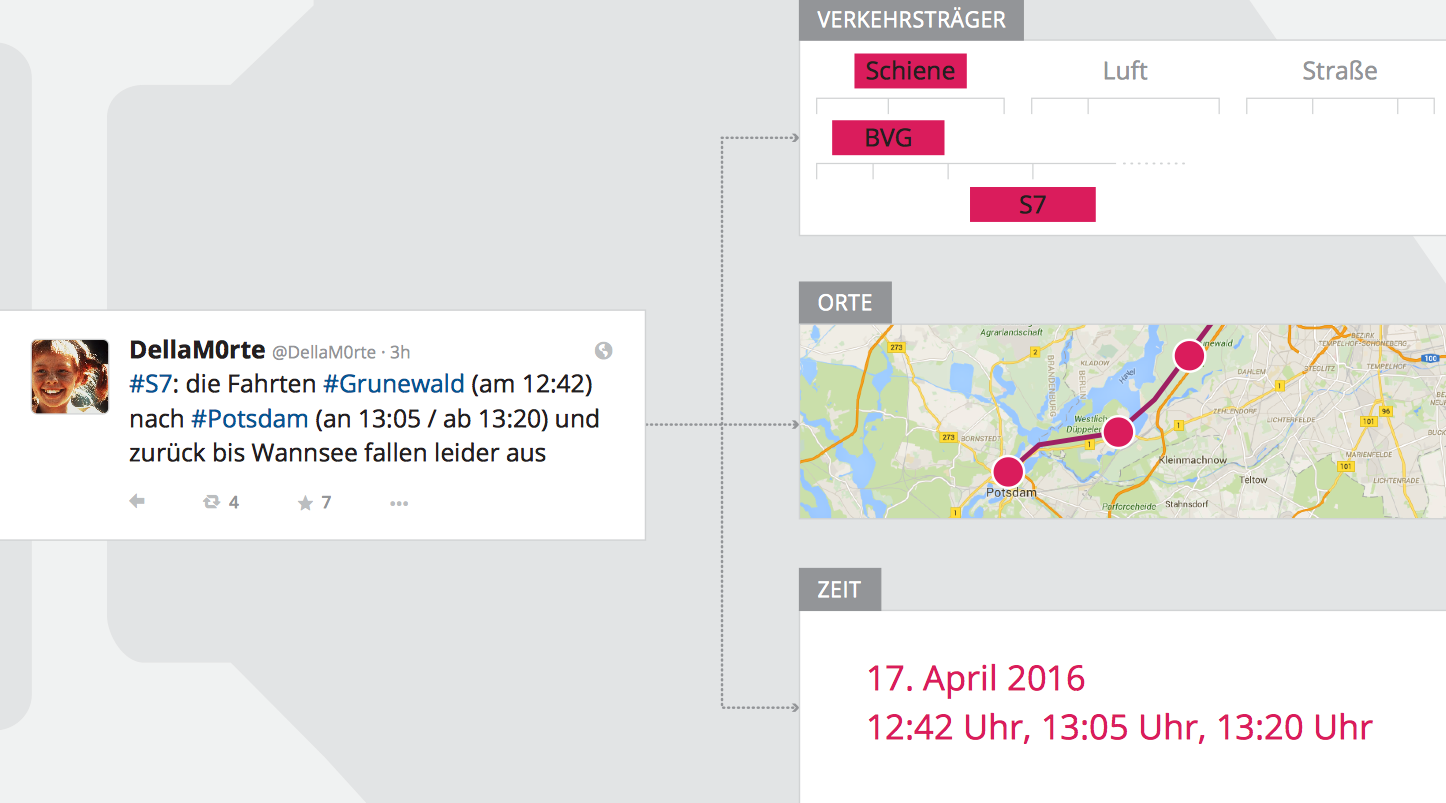
\includegraphics[width=1\textwidth]{gfx/sd4m_praesi_1.png}}
   \caption{Verknüpfung eines Tweets mit Fahrplandaten\protect\cite{WEB:SD4M:Presentation:2016}}
   \label{fig:tweetXfahrplan}
 \end{figure}

\section{Vorbereitung der Arbeitsumgebung}
\label{sec:main:preparation}
Eigener Rechner, lokale Umgebung, DB ... warum?



\section{Einarbeitung}
\section{Aufgaben}
\subsection{Extraktion einer Straßenliste}
\subsection{Verknüpfung von Daten der Deutschen Bahn mit Daten aus OpenStreetMap}
\subsection{Datenaufwertung??}
